\documentclass[14pt]{extarticle}
\usepackage[utf8]{inputenc}
\usepackage{ngerman}
\usepackage{array}
\usepackage{amsmath}
\usepackage{graphicx}
\title{Bericht Todesstern U2}
\author{Charline Waldrich, Robert Ullmann, Julian Dobrot}
\date{13. november 2015}

\begin{document}

\maketitle
\pagebreak
\tableofcontents


\section{Aufgabenstellung}

\subsection{Strahl}
Die Klasse Ray representiert einen Strahl. Im konstruktor dieser Klasse soll der Ursprung und die Richtung des Strahls übergeben werden.  
\subsection{Kameras}
Es sollen drei Kameraklassen implementiert werden. 
\subsubsection{Camera}
Diese Klasse ist die abstrakte Basisklasse. sie speichert die drei Vektoren e,g,t welche im Konstruktor übergeben werden. Außerdem 
wird die Kameratransformation der vektoren u,v,w auch in ihrem Konstruktor berechnet.
\subsubsection{OrthographicCamera}
Soll eine orthogrsphische Kamera wiederspiegeln und hat als weiteren Parameter den Skalierungsfaktor der bildebene.
\subsubsection{PespectiveCamera}
Eine perspektivische Kamera mit dem Öffnungswinkel als weiterem Parameter 

\subsection{Farben}
Die Klasse Farben soll Farben im RGB-Farbraum representieren. Dabei sollen die einzelnen Komponenten einen Wert von 0 und 1 annehmen. Farben sollen addiert, subtrahiert und multipliziert werden. Desweiteren sollen Farben mit einem skalar mutlipliziert werden können.

\subsection{Geometrien}
Alle Geometrien erben von einer abstrakten Basisklasse. Diese hat nur ein Attribut nämlich die Farbe. 
\subsubsection{Hit}
\subsubsection{Plane}
Die Klasse Plane soll eine Implementierung einer Ebenel darstellen. 
\subsubsection{Sphere}
Die Klasse Sphere soll eine Implementierung einer Kugel darstellen. 
\subsubsection{Triangle}
Die Klasse Triangle soll eine Implementierung eines Dreicks darstellen. 
\subsubsection{AxisAlignedBox}
Die Klasse Sphere soll eine Implementierung einer Box darstellen. 
\subsection{Welt}
In der Welt sollen die darzustellenden Objekte in einer Scene dargestellt werden
\subsection{Raytracer}
Hier soll über jeden pixel des Bildes iteriert werden. Werden Schnittpunkte mit Geometrien gefunden, erhält der Pixel dessen Farbe.


\section{Lösungsstrategien}
Allgemein wurden als erster Lösungsschritt alle aus der Aufgabenstllung hervorgehenden Klassendiagramme komplett in das Projekt integriert.

\subsection{Strahl}
\subsection{Kameras}
\subsubsection{Camera}
Die Kamera führt die Transformation der Position, Richtung und Rotation durch.
\subsubsection{OrthographicCamera}
Bei der Orhographischen Kamera müssen alle erzeugten Strahlen parallel sein und in die gleiche Richtung zeigen.
\subsubsection{PespectiveCamera}  
\subsection{Farben}
Die Klasse der Farbe, repräsentiert eine Farbe, welche ein neues Objekt vom Typ Color erzeugen kann.
\subsection{Geometrien}
\subsubsection{Hit}
\subsubsection{Plane}
\subsubsection{Sphere}
Als Lösungsansatz für diese Geometrie dienten die aus der Vorlesung erarbeite Formel zur berechnung der Schnittpunkte verwendet.
\\\\\begin{math} t=\frac{-b\pm \sqrt[2]{b^2-4ac}}{2a}\end{math}\\\\
Für die berechnung der Anzahl der Schnittpunkte mit der Sphäre wurde die folgende Formel herangezohgen:
\\\\\begin{math} d=b^2-4ac\end{math}\\\\
Wobei der Strahl bei \begin{math}d < 0\end{math} keinen Schnittpunkt mit der Kugel aufweist. Bei \begin{math}d = 0\end{math} genau einen und bei \begin{math}d > 0\end{math} zwei Schnittpunkte.\\
Die einzelnen Komponennten dieser formeln setzen sich wie folgt zusammen:\\\\
\begin{math}a=d^2\end{math}\\\\
\begin{math}b=d*[2(o-c)]\end{math}\\\\
\begin{math}c=(o-c)*(o-c)-r^2\end{math}\\\\

Diese Überlegungen wurden dementsprechend programmtechnisch umgesetzt, um eine gewünschte implementierung der hit-Methode zu erzielen.
 

\subsubsection{Triangle}
Die Triangle besteht aus 3 Punkten, welche die Baryzentrischen Koordinaten bilden. Um den Schnittpunkt zu berechnen, ist es notwenig mit Hilfe der 3x3 Matrix ein lineares Gleichungssystem zu erstellen und es mit der Cramerschen Regel, unter Verwendung der Determinanten aus der 3x3 Matrix zu lösen.
\subsubsection{AxisAlignedBox}

\subsection{Welt}
\subsection{Raytracer}

\section{Implementierungen}

\subsection{Strahl}
Die ,,Ray'' Klasse initialisiert einen Strahl mit gegebenem Ausgangspunkt und Richtungsvektor. Sie implementiert zwei Methoden namens ,,at'' und ,,tOf''. Außerdem wurden die von der Oberklasse Object geerbten Methoden hashCode und eqals so überschrieben, dass sie zum Testen nützlich sind.\\
Der Strahl (Ray) kann mit der Methode ,,at'' den Punkt berechnen, welchen er trifft wenn er die als Parameter übergebenen Länge ,,t'' (als double Wert), den Richtungsvektor ''entlang geht''. Hierfür wird die eine einfache Rechnung angewandt. 
%$$ Punt P = Ausgangspunkt O + Länge t \times Richtungsvektor d $$
In der Methode ,,tOf'' wird diese Rechnung umgedreht. Ein gesuchter Punkt wird als Parameter übergeben und berechnet dann den Faktor ,,t'' (als double Wert) welcher mit dem Richtungsvektor multipliziert werden müsste um zu gesuchtem Punkt zu gelangen. \\
\subsection{Kameras}
\subsubsection{Camera}
\subsubsection{OrthographicCamera}
Die Klasse OrthographicCamera  bekommt 2 Vektoren und einen Punkt übergeben, zusätzllch noch den Öffnungswinkel. In der öffentlichen Methode rayfor, wird der sichtbare Bereich in Höhe und Breite festgelegt und mit Hilfe der Formel der Orthographischen Kamera der Strahl zurückgegeben, welcher für die Projektion notwendig ist.
\subsubsection{PespectiveCamera}
\subsection{Farben}
Die übergebenen Variablen vom Typ double stehen für die Farben Rot, Gelb , Blau und werden im Konstruktur dem Objekt selbst übergeben.
\subsection{Geometrien}

\subsubsection{Hit}
Das Hit Objekt bekommt einen double Wert ,,t'', einen Strahl ,,ray'' und eine geometrische Figur übergeben und zugewiesen. Außerdem werden in der Klasse die von der Oberklasse Object vererbten Methoden ,,toString'', ,,hashCode'' und ,,equals'' überschrieben.
\subsubsection{Plane}
\subsubsection{Sphere}
\subsubsection{Triangle}
Zu Beginn werden die Übergebenen Variablen auf Plausibilität geprüft, danach wird das linierae GLeichungssystem mithilfe einer Matrix aus der Matrix-Vektor-Bibliothek erstellt. Im folgenden wird druch das tauschen der Zeilen einer der Faktoren eliminiert. Am Ende kann mit Hilfe der Cramerschen Regel und den Determinanten der Matrizen $\beta$ , $\gamma$ und $t$ bestimmt werden.
\subsubsection{AxisAlignedBox}
\subsubsection{Plane}

Die Klasse Plane beschreibt eine Ebene. Diese wird genau definiert durch die übergebenen Parameter; einen auf der Ebene liegenden Punkt, einem Normalen-Vektor welcher die Ausrichtung (bzw. Neigung) der Ebene definiert, und einem Color Objekt welche die Farbe der Ebene hält. \\
Die von der Oberklasse Object geerbten Methoden ,,toString'', ,,hashCode'' und ,,equals'' wurden sinnvoll überschrieben.\\
Des weiteren wird die Methode ,,hit'' von der abstrakten Oberklasse Geometry vererbt und auf die Ebene angepasst. Diese bekommt einen Strahl übergeben welcher nicht null sein darf und gibt ein Hit Objekt zurück. Danach wird zunächst getestet ob das Skalarprodukt des Strahls und des Normalenvektor gleich Null ist. Ist dies der Fall sind Ebene und Strahl paralell und ,,null'' wird zurück gegeben. \\
Ist dies nicht der Fall, wird für den Strahl und die Ebene die Entfernung berechnet. \\
Ist diese kleiner Null bedeutet das, dass das Objekt vor dem Ortsvektor des Strahls (und somit vor unserer Bildschirmfläche) liegt und es wird wieder ein ,,null'' Objekt zurück geliefert. \\
Ist der berechnete double-Wert größer 0 wird ein Hit Objekt mit dem berechneten ,,t''-Wert, dem der Methode übergebenen Ray ,,r'' und der im Konstruktor zugewiesenen Farbe zurück gegeben (siehe Abb. \ref{Ebene}).\\
Außerdem wird in unserer Color Klasse der RGB-Wert berechnet, welcher für das färben des writableImage Objektes nicht brauchbar ist. Da der pixelWriter nur Color Objet aus dem javaFX Paket erkennt, müssen die einzeln berechneten Werte an ein neues Color Objekt dessen übergeben werden.
\begin{figure}[ht]
\begin{center}
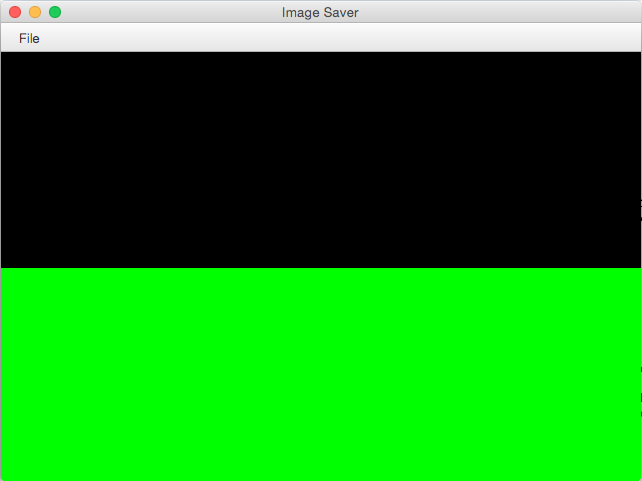
\includegraphics[width=5cm, height=8cm]{TestCase1.png}
\caption{Ebene aus Perspektivischer Kamera}
\label{Ebene}
\end{center}
\end{figure}


\subsection{Welt}

Die Klasse ,,World'' initialisiert ein Fenster mit übergebener Hintergrundfarbe. Diese soll zukünftig vom Nutzer ausgewählt werden. Sie beinhaltet eine Array Liste in welcher nur Objekte des Typs ,,Geometry'' gespeichert werden können.\\ 
Des weiteren gibt es eine Methode namens ,,hit'' welche einen Strahl (Ray) übergeben bekommt und eine Farbe vom Typ Color zurück gibt. Zunächst wird ein Hit Objekt ,,hit0'' der mit dem null-Wert initialisiert. \\
In der for-Schleife wird für jedes Objekt in der Liste ein weiteres Hit Objekt mit dem übergebenen Strahl gespeichert. Hält das ,,hit1'' Objekt einen Wert welcher ungleich null ist und liegt vor den anderen Objekten (hat also ein kleineren ,,t''-Wert, als die Objekte welche davor in hit0 gespeichert wurden), so wird der außen liegenden Variable ,,hit0'' dieses Hit Objekt zugewiesen. Sollte nach dem Durchgang der kompletten Schleife der Wert von ,,hit0'' immer noch null sein, so wird die Hintergrundfarbe der Welt zurück gegeben. Wenn nicht so wird immer die Farbe des am nächstliegendsten Objekt zurück gegeben. 

\subsection{Raytracer}



\section{Besondere Probleme oder Schwierigkeiten bei der Bearbeitung}

\subsection{Strahl}
\subsection{Kameras}
\subsubsection{Camera}
Ein Fehler in der Camera klasse führte zueiner überarbeitung der Cameratransformation, da Koordinaten falsch berechnetwurden, kam es bem Rendering der Box zu foldendem Ergebniss.\\
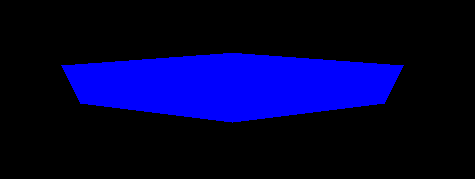
\includegraphics{BoxFail}

\subsubsection{OrthographicCamera}
Problem bei der Implementierung ist die späte Feststellung, ob die Kamera richtig Implementiert wurde, da ein Debuggen nur bedingt möglich ist, da sehr viele Straheln (Ray) erzeugt werden.
\subsubsection{PespectiveCamera}
\subsection{Farben}
\subsection{Geometrien}
\subsubsection{Hit}
\subsubsection{Plane}
\subsubsection{Sphere}
Ein Fehler in einer der Methoden der Klasse Vector3 führte zu einer längeren Fehlersuche. Durch einen Operatorschreibfehler kam es zu einer Fehlerhaften berechnung wie im folgendem Bild zu sehen ist:\\\\
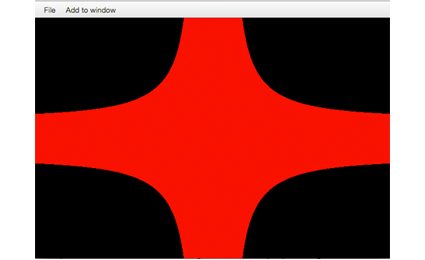
\includegraphics{KugelFail}
\subsubsection{Triangle}
Große Probleme bei der Implementierung der Klasse Triangle, gab es beim Verständnis der Formel und der richtigen Implementierung in Java-Code. Auch mögliche Fehler in der Vektor-Bibliothek führten zu nicht gleich offensichtlichen Problemen. 
\subsubsection{AxisAlignedBox}

\subsection{Welt}
\subsection{Raytracer}

In der ImageSaver Klasse musste die ,,getColor''-Methode angepasst werden. Diese benutzt unsere persönliche Color Klasse und berechnet für jeden einzelnen Pixel dank der ,,hit'' Methode der Welt, ob das erzeugte Objekt von dem Strahl der erzeugten Klasse getroffen wird. Da in der Bildverarbeitung der Ursprung des Koordinatensystems oben links und in der Mathematik unten links liegt, musste bei der Berechnung aufgepasst werden, dass der ,,rayFor'' Methode welche von der ,,camera'' aufgerufen wird. nicht die oben liegende Y-Koordinate übergeben wird, sondern dem quasi spiegelverkehrtem Pixel unten. 

-> hier kannst du rein schreiben was bei der Camera Klasse das Problem war und wie es schön das ganze Projekt kaputt gemacht hat ;) 



\section{Zeitbedarf}
\begin{center}
\begin{tabular}{cr}
Strahl	  \	&80 min	\\
Kameras 	\	&240 min	\\
Farben \	&240 min	\\
Geometrien \	&240 min	\\
Welt \	&240 min	\\
Raytracer \	&240 min	\\

Bericht  \		&180 min	 \\
	\hline
	&740 min
\end{tabular}
\end{center}

\subsection{Tests}

\section{Quellen}
https://asalga.wordpress.com/2012/09/23/understanding-vector-reflection-visually/





\end{document}
